% !TeX spellcheck = en_GB
\section{Observations at the weather mast}
\label{sec:loc_obs}
The large scale synoptic analysis will be related to the local weather  observations at Haukeliseter. 
\\
\SI{60}{\minute} accumulation is presented as bars in \Cref{fig:TPU} and will show the continuous precipitation at Haukeliseter during the extreme event. The possible change of precipitation will be investigated with the temperature. Snow fall is likely for temperatures up to \SI{2}{\celsius}. The intensity of the storm can be classified by the hourly averaged wind speed and direction as wind barbs in \SI{}{\mPs}.
To understand which damage a storm can have, \cite{faeraas_urd_2016} released a table to associate wind strength with damage (see \Cref{tab:wind}).
%%% Damage related to wind speed %%%%%%%%%%%%%%%%%%%%%%%%%%%%%%%%%%%%%
% !TeX spellcheck = en_GB
\begin{table}[h!]
	\begin{center}
		\caption{Damage related to wind speed, from \cite{faeraas_urd_2016}. }\label{tab:wind}
		\begin{tabular}{l|c|l}
			\hline \hline
			slight storm& \SI{20.8}{\mPs} -- \SI{24.4}{\mPs}&  Large trees sway and hiver. \\
			&  &  Roofs can blow down. \\ \hline
			full storm & \SI{24.5}{\mPs} -- \SI{28.4}{\mPs}& Trees are pulled up with clutter. \\
			&  & Big damages to houses.\\ \hline
			strong storm & \SI{28.5}{\mPs} -- \SI{32.6}{\mPs}& Extensive damage.\\
			&  & \\ \hline
			hurricane & \textgreater \SI{32.6}{\mPs}& Unusually large destruction.\\
			\hline \hline
		\end{tabular}
	\end{center}
\end{table}
%%%%%%%%%%%%%%%%%%%%%%%%%%%%%%%%%%%%%%%%%%%%%%%%%%%%%%%%%%%%%%%%%%%%%%%%%%
%%% local observations @ Haukeliseter %%%%%%%%%%%%%%%%%%%%%%%%%%%%%%%%%%%%%
% !TeX spellcheck = en_GB
\begin{figure}[h!]
	\centering
	%%%%%% 20/12
	\begin{subfigure}[b]{0.49\textwidth}
		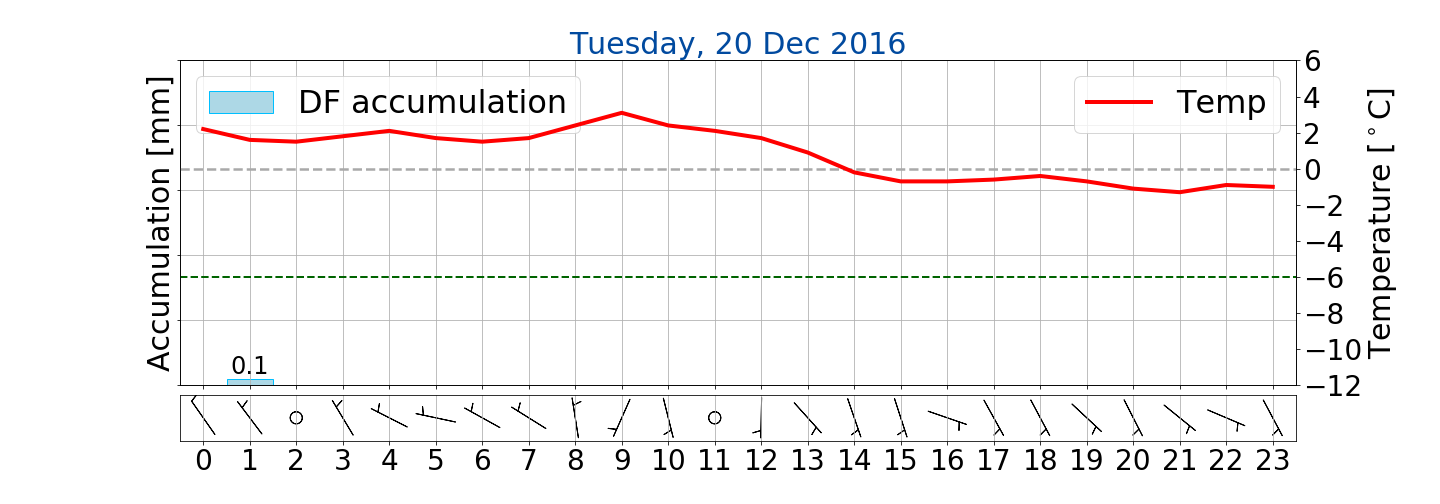
\includegraphics[trim={4.9cm 1.cm 1.5cm 1cm},clip,
		width=\textwidth]{./fig_weathermast/T_P_U_20161220}
		\caption{}\label{fig:TPU20}
	\end{subfigure}
	\hfill
	%%%%%% 21/12
	\begin{subfigure}[b]{0.49\textwidth}
		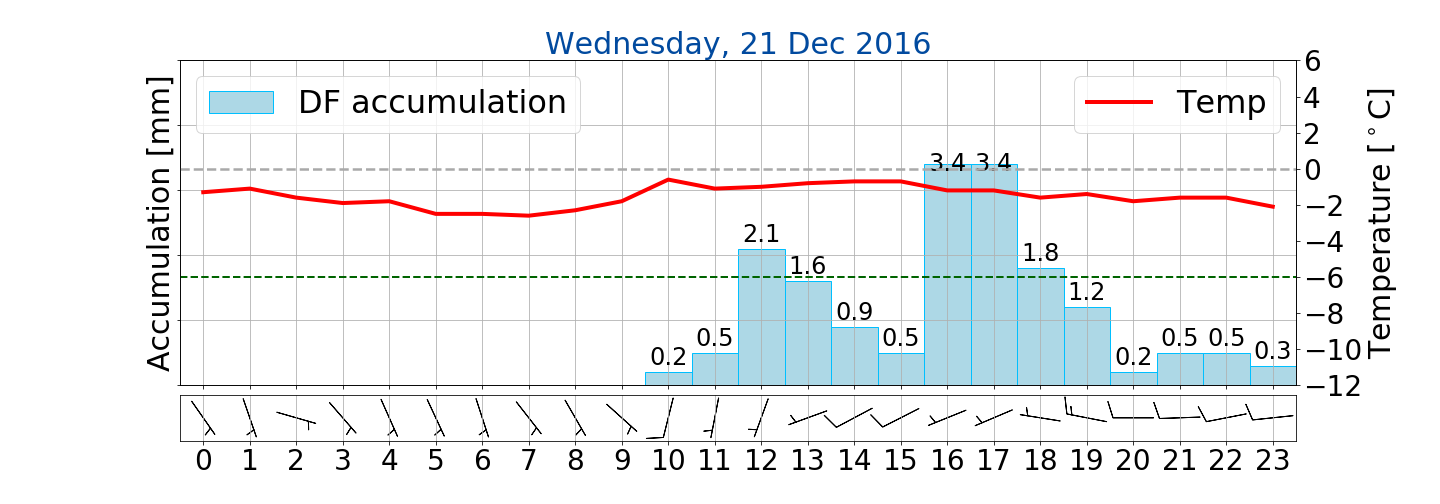
\includegraphics[trim={4.9cm 1.cm 1.5cm 1cm},clip,
		width=\textwidth]{./fig_weathermast/T_P_U_20161221}
		\caption{}\label{fig:TPU21}
	\end{subfigure}
% \end{figure}
% \begin{figure}\ContinuedFloat
	\centering
	%%%%%% 22/12
	\begin{subfigure}[b]{0.49\textwidth}
		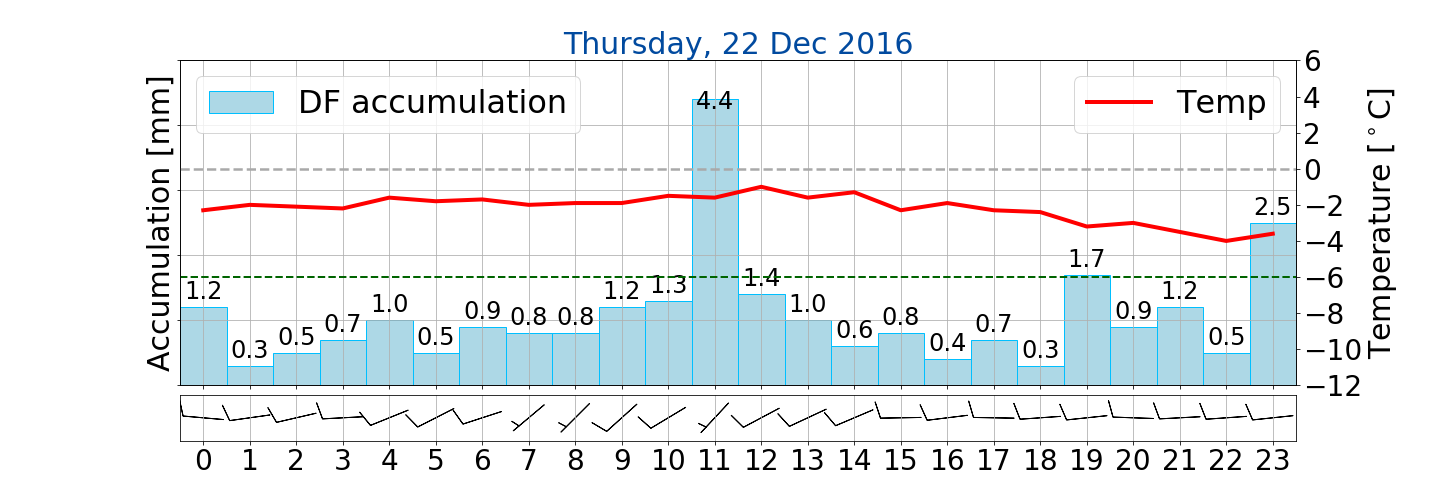
\includegraphics[trim={4.9cm 1.cm 1.5cm 1cm},clip,
		width=\textwidth]{./fig_weathermast/T_P_U_20161222}
		\caption{}\label{fig:TPU22}
	\end{subfigure}
	\hfill
	%%%%%% 23/12
	\begin{subfigure}[b]{0.49\textwidth}
		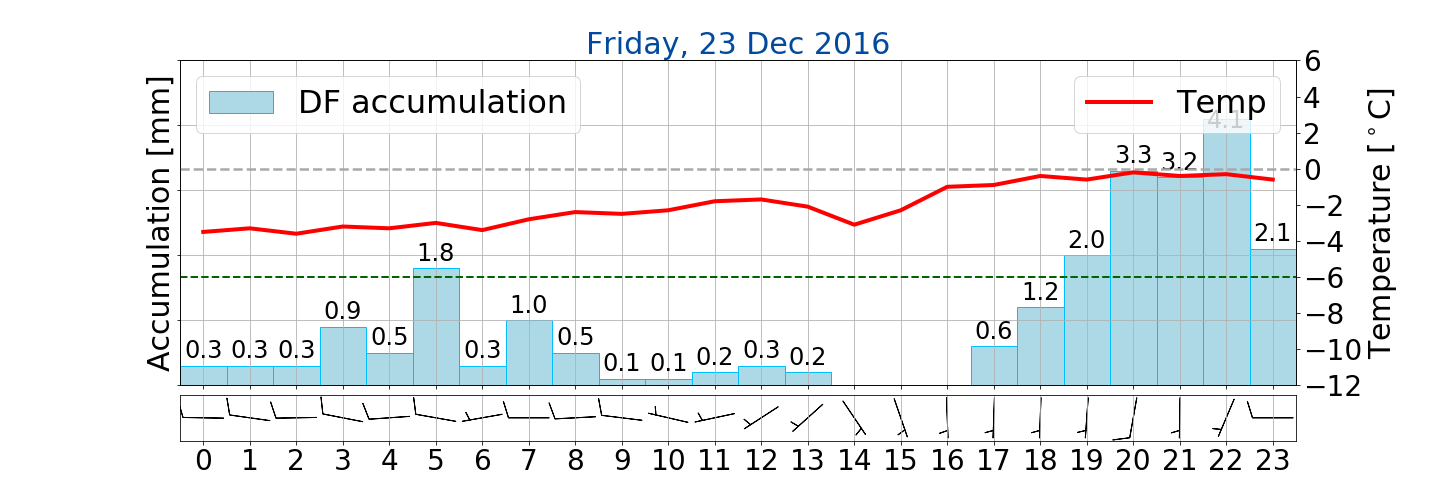
\includegraphics[trim={4.9cm 1.cm 1.5cm 1cm},clip,
		width=\textwidth]{./fig_weathermast/T_P_U_20161223}
		\caption{}\label{fig:TPU23}
	\end{subfigure}
	%\end{figure}
	%\begin{figure}[h]\ContinuedFloat
	%%%%%% 24/12
	\begin{subfigure}[b]{0.49\textwidth}
		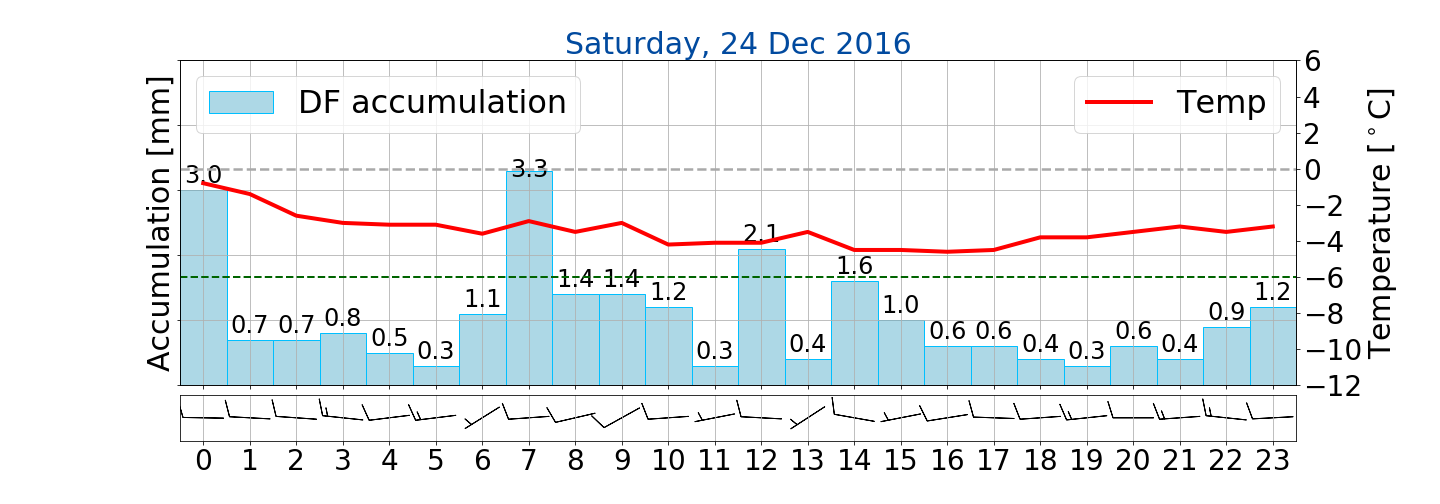
\includegraphics[trim={4.9cm 1.cm 1.5cm 1cm},clip,
		width=\textwidth]{./fig_weathermast/T_P_U_20161224}
		\caption{}\label{fig:TPU24}
	\end{subfigure}
	\hfill
	%%%%%% 25/12
	\begin{subfigure}[b]{0.49\textwidth}
		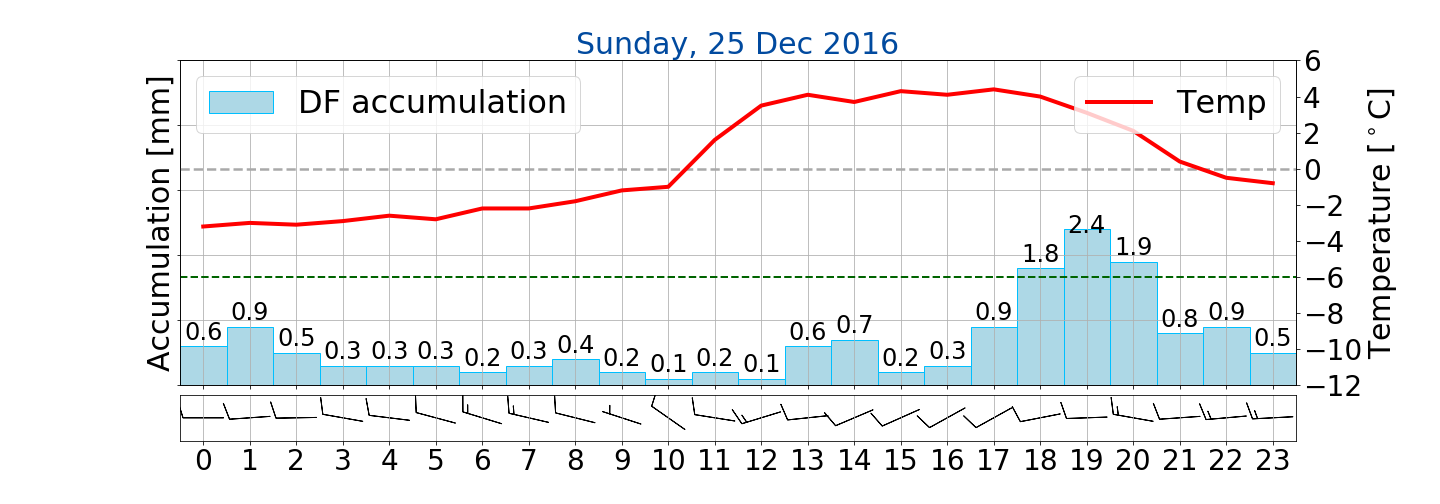
\includegraphics[trim={4.9cm 1.cm 1.5cm 1cm},clip,
		width=\textwidth]{./fig_weathermast/T_P_U_20161225}
		\caption{}\label{fig:TPU25}
	\end{subfigure}
	%%%%%% 26/12
	\begin{subfigure}[b]{0.49\textwidth}
		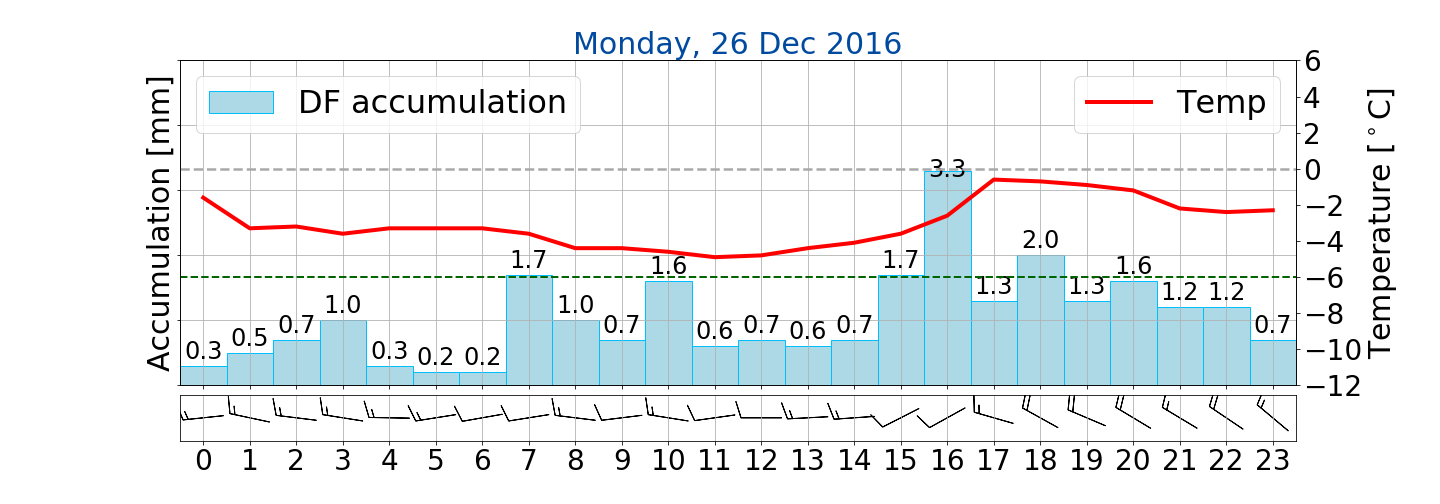
\includegraphics[trim={4.9cm 1.cm 1.5cm 1cm},clip,
		width=\textwidth]{./fig_weathermast/T_P_U_20161226}
		\caption{}\label{fig:TPU26}
	\end{subfigure}
	\hfill
	%%%%%% 27/12
	\begin{subfigure}[b]{0.49\textwidth}
		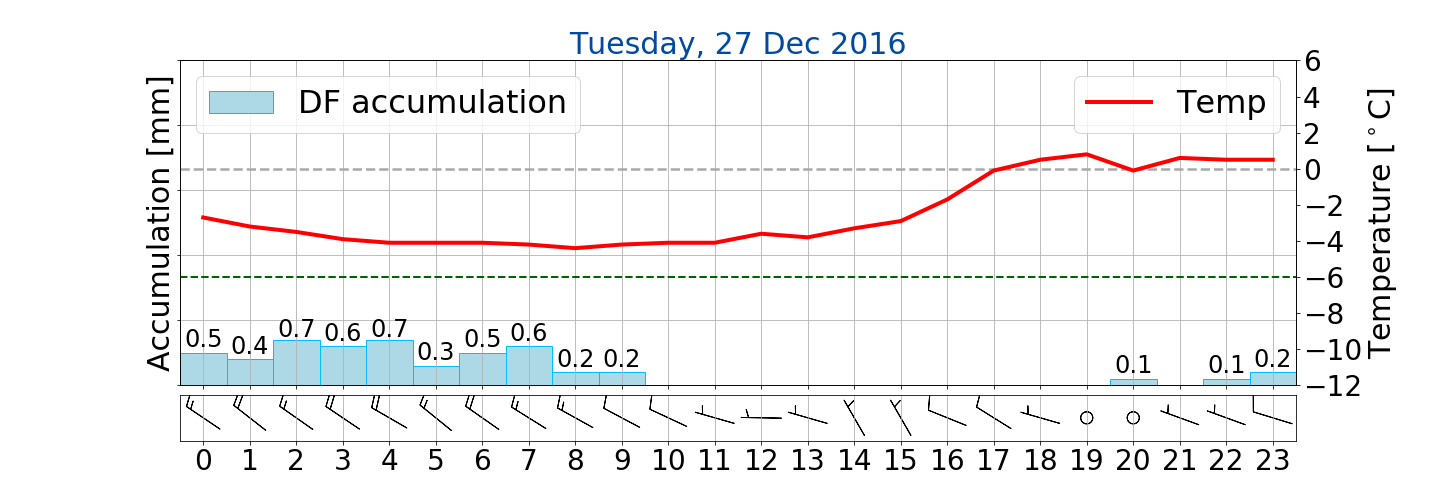
\includegraphics[trim={4.9cm 1.cm 1.5cm 1cm},clip,
		width=\textwidth]{./fig_weathermast/T_P_U_20161227}
		\caption{}\label{fig:TPU27}
	\end{subfigure}
	\caption{Observation from the weather mast at Haukeliseter during \SIrange{20}{27}{\dec}. \SI{60}{\minute} total accumulation [\SI{}{\mm}] in light blue as bar, temperature (red, [\SI{}{\celsius}]), and wind as barbs [\SI{}{\mPs}]. Gray dashed line indicates the freezing temperature and the green dashed line the 30-year climate mean temperature at \SI{-6}{\celsius}. Hourly processed data taken from \cite{eklima_norwegian_2016}.} \label{fig:TPU}
\end{figure}
%%%%%%%%%%%%%%%%%%%%%%%%%%%%%%%%%%%%%%%%%%%%%%%%%%%%%%%%%%%%%%%%%%%%%%%%%%